\section{Tartószerkezet és 3D nyomtatott váz}

A drónok tervezése és építése során az egyik legfontosabb szempont a stabil és megbízható tartószerkezet kialakítása. Az alkalmazott anyagok és technológiák döntően befolyásolják a drón repülési jellemzőit, terhelhetőségét és élettartamát. A projektünk során a 3D nyomtatási technológiát választottuk a váz és a tartószerkezet létrehozásához, mivel ez a módszer számos előnyt kínál a hagyományos gyártási technikákkal szemben.

Az alkalmazott 3D nyomtatási technológia lehetővé teszi a komplex geometriák és precíz részletek létrehozását, amelyek különösen fontosak a drón szerkezetének optimalizálása és a súlycsökkentés szempontjából. A 3D nyomtatott váz könnyű, mégis rendkívül erős, ami hozzájárul a drón stabil repülési tulajdonságaihoz és hosszú élettartamához.

A drón vázát 70%-os kitöltéssel nyomtattuk PET-G anyagból, amely erős és ellenálló, miközben megőrzi a szükséges rugalmasságot és könnyűséget. Az egyes aklatrészek rögzítése egymáshoz 16 darab M5-ös 20 miliméteres hexagon fejű csavarral és M5-ös anyával történt. 

\begin{figure}[H]
	\centering
	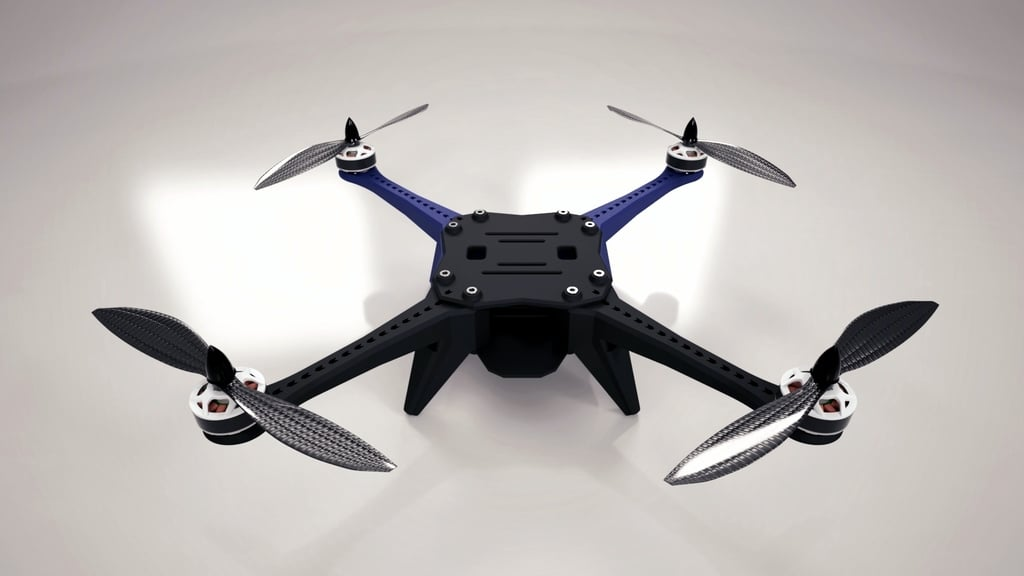
\includegraphics[scale=0.3]{figures/drone_model.JPG}
	\caption{A drón 3D -s modellje}
	\label{A drón 3D -s modellje}
\end{figure}

